\documentclass{beamer}

\mode<presentation> {
	
	% The Beamer class comes with a number of default slide themes
	% which change the colors and layouts of slides. Below this is a list
	% of all the themes, uncomment each in turn to see what they look like.
	
	%\usetheme{default}
	%\usetheme{AnnArbor}
	%\usetheme{Antibes}
	%\usetheme{Bergen}
	%\usetheme{Berkeley}
	%\usetheme{Berlin}
	%\usetheme{Boadilla}
	%\usetheme{CambridgeUS}
	%\usetheme{Copenhagen}
	%\usetheme{Darmstadt}
	%\usetheme{Dresden}
	%\usetheme{Frankfurt}
	%\usetheme{Goettingen}
	%\usetheme{Hannover}
	%\usetheme{Ilmenau}
	%\usetheme{JuanLesPins}
	%\usetheme{Luebeck}
	\usetheme{Madrid}
	%\usetheme{Malmoe}
	%\usetheme{Marburg}
	%\usetheme{Montpellier}
	%\usetheme{PaloAlto}
	%\usetheme{Pittsburgh}
	%\usetheme{Rochester}
	%\usetheme{Singapore}
	%\usetheme{Szeged}
	%\usetheme{Warsaw}
	
	% As well as themes, the Beamer class has a number of color themes
	% for any slide theme. Uncomment each of these in turn to see how it
	% changes the colors of your current slide theme.
	
	%\usecolortheme{albatross}
	%\usecolortheme{beaver}
	%\usecolortheme{beetle}
	%\usecolortheme{crane}
	%\usecolortheme{dolphin}
	%\usecolortheme{dove}
	%\usecolortheme{fly}
	%\usecolortheme{lily}
	%\usecolortheme{orchid}
	%\usecolortheme{rose}
	%\usecolortheme{seagull}
	%\usecolortheme{seahorse}
	%\usecolortheme{whale}
	%\usecolortheme{wolverine}
	
	%\setbeamertemplate{footline} % To remove the footer line in all slides uncomment this line
	%\setbeamertemplate{footline}[page number] % To replace the footer line in all slides with a simple slide count uncomment this line
	
	%\setbeamertemplate{navigation symbols}{} % To remove the navigation symbols from the bottom of all slides uncomment this line
}

\usepackage{graphicx} % Allows including images
\usepackage{booktabs} % Allows the use of \toprule, \midrule and \bottomrule in tables 

\usepackage[T1]{fontenc}
\usepackage[utf8]{inputenc}
\setbeamertemplate{caption}[numbered]
\newcommand{\C}{\mathbb{C}}
\newcommand{\R}{\mathbb{R}}
\newcommand{\Q}{\mathbb{Q}}
\newcommand{\Z}{\mathbb{Z}}
\newcommand{\N}{\mathbb{N}}
\newcommand{\p}{\mathbb{P}}
\newcommand{\E}{\mathbb{E}}
\usepackage{graphicx}
\usepackage{amssymb}
\usepackage{setspace}
\usepackage[toc,page]{appendix}
\usepackage{epstopdf}
\usepackage{latexsym}
\usepackage{amstext}
\usepackage{lmodern}
\usepackage{amsmath}
\usepackage{bbm}
\usepackage{amsfonts}
\usepackage{url}
\usepackage{bm}
\usepackage{mathrsfs}
\usepackage{mathtools}
\usepackage{float}
%\usepackage{hyperref} give reference hyperlink 
%\usepackage{setspace}
\usepackage{indentfirst}
\usepackage{multirow}
\usepackage{color}
\usepackage{mathtools}
% packages from template
\usepackage{amsmath,amsthm,amssymb,amsfonts}
\usepackage[width=.9\textwidth]{caption}
\usepackage{mathrsfs}
\usepackage{graphicx}
\newcommand{\indep}{\rotatebox[origin=c]{90}{$\models$}}
\usepackage{textgreek}
\usepackage{bbold}
\usepackage{subcaption}
\usepackage{natbib}
\usepackage{verbatim}
\usepackage{soul}
\usepackage[utf8]{inputenc}
\usepackage[algo2e,ruled,vlined]{algorithm2e} 
\usepackage{fancyvrb}


\newtheorem{proposition}[theorem]{Proposition}

\newcommand{\M}{\mathbf{M}}
\newcommand{\rank}{\mathrm{rank}}
\newcommand{\rep}{\mathrm{rep}}
\newcommand{\PR}{\text{Pr}}
\newcommand{\pkg}[1]{{\fontseries{b}\selectfont #1}}
%\newcommand\norm[1]{\left\lVert#1\right\rVert}
\newcommand{\bs}[1]{\pmb{#1}}
\newcommand{\mb}[1]{\mathbf{#1}}
\DeclareMathOperator*{\argmin}{arg\,min}
\DeclarePairedDelimiter{\ceil}{\lceil}{\rceil}
\DeclarePairedDelimiterX{\norm}[1]{\lVert}{\rVert}{#1}
\allowdisplaybreaks
%=============================================================================
% prelude
%=============================================================================
\def\mathLarge#1{\mbox{\LARGE $#1$}}
\usepackage{soul}


\title[]{Topics in Image-based Prognosis}
\author[Hongda Zhang]{Hongda Zhang}
\institute{Nanjing University}
\date{\today}



\begin{document}
	\begin{frame}
		\titlepage
	\end{frame}
	
	\begin{frame}
		\frametitle{Contents}
		\begin{enumerate}
			\item Whole slide images based cancer survival prediction using attention guided deep multiple instance learning networks
			\item Predicting cancer outcomes from histology and genomics using convolutional networks
		\end{enumerate}
		\nocite{*}
	\end{frame}
	
	\begin{frame}
		\frametitle{DeepAttnMISL}
		Contributions \\
		\vspace{5mm}
		The Deep Attention Multiple-Instance Survival Learning (DeepAttnMISL) is proposed to make accurate prognosis for cancer patients using whole slide images. The main contributions are shown below:
		\begin{itemize}
			\item The proposed multiple instance deep neural network first extract instance-level features from a number of patches through a Siamese MIL-based network. Then features from multiple instances are aggregated according to the attentions. The multiple instance framework solve the problem that each patient have many image patches used for prognosis. Using each patch as if it is from a separate individual may cause bias since the number of patches of different patients varies. In contrast, the multiple instance framework aggregates features from multiple patches to one patient-level feature. Moreover, the attention based feature aggregation is more flexible than fixed pooling operations, e.g. max pooling, and helps make better prognosis. 
		\end{itemize}
	\end{frame}
	
	\begin{frame}
		\frametitle{DeepAttnMISL}
		Contributions (cont.) 
		\begin{itemize}
			\item The proposed model is useful for finding prognosis relevant patches from the whole slide images. The relevance of the instances are compared using the calculated attentions. The set of patches of an instance with greater value of attention are considered more relevant to prognosis.
			\item Extensive experiments are conducted on two large datasets to access the performance of the proposed framework. One dataset is from National Lung Screening Trial (NLST) and the other is from the Molecular and Cellular Oncology (MCO) study.
		\end{itemize}
	\end{frame}

	\begin{frame}
		\frametitle{DeepAttnMISL}
		Contributions (cont.)
		\begin{figure}[H]
			\centering
			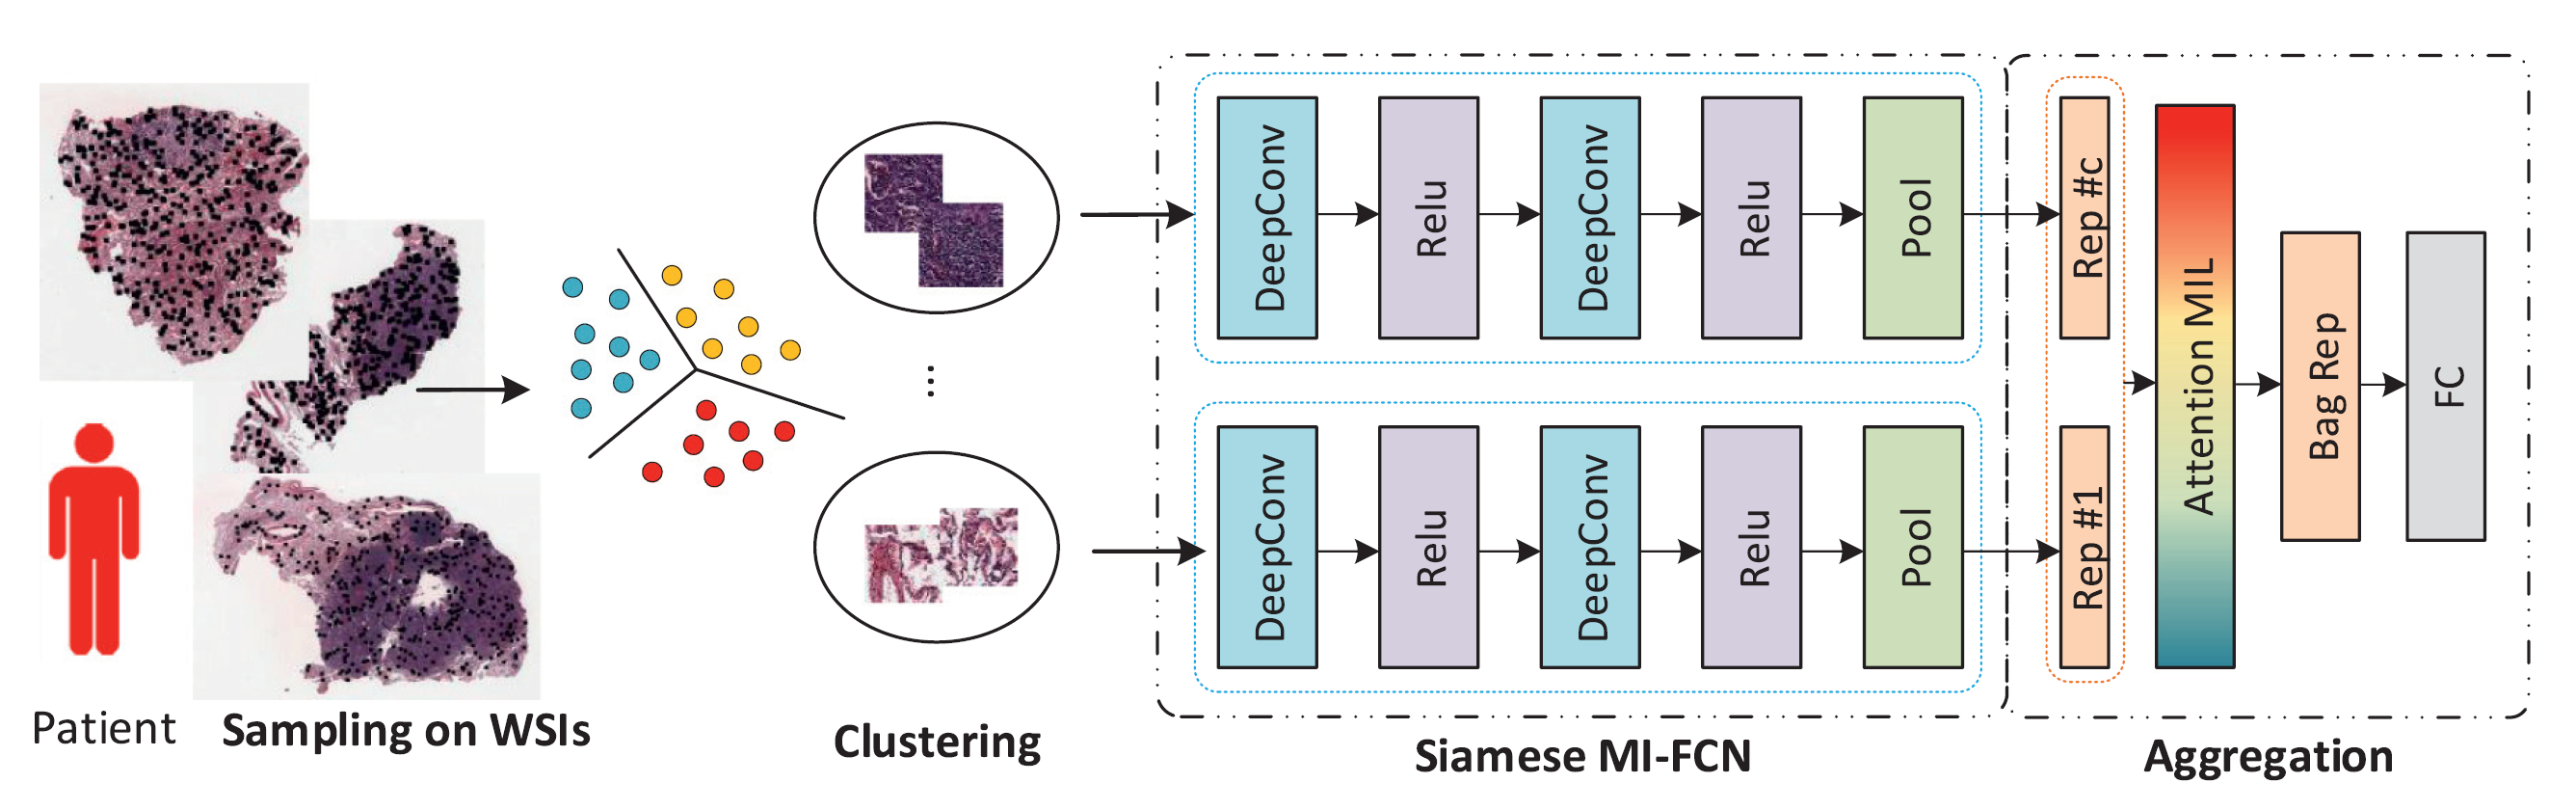
\includegraphics[scale=0.12]{figures/full.png}
			\caption{Overall structure of the proposed framework.}
			\label{fig:full}
		\end{figure}
	\end{frame}
	
	\begin{frame}
		\frametitle{DeepAttnMISL}
		Contributions (cont.) 
		
		\begin{figure}[H]
			\centering
			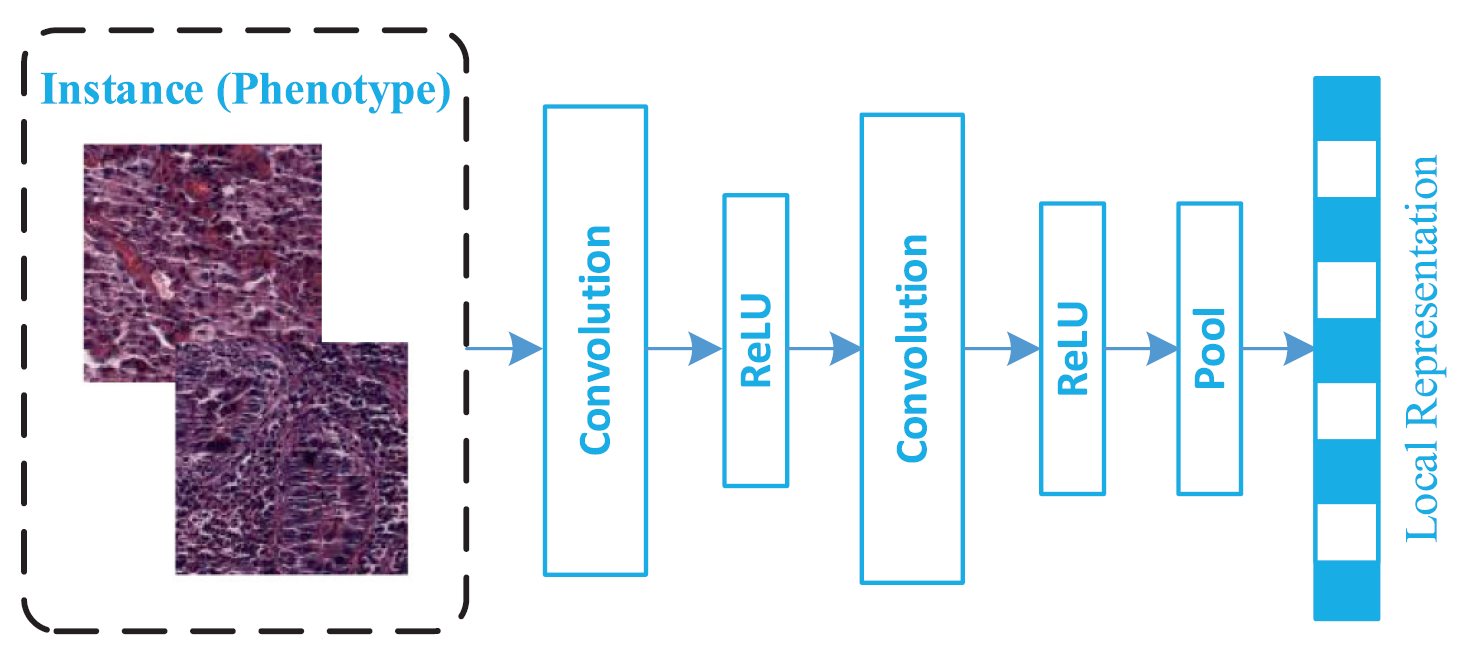
\includegraphics[scale=0.20]{figures/part.png}
			\caption{Structure of each MI-FCN.}
			\label{fig:part}
		\end{figure}
	\end{frame}
	
	\begin{frame}
		\frametitle{DeepAttnMISL}
		Contributions (cont.)
		
		\begin{figure}[H]
			\centering
			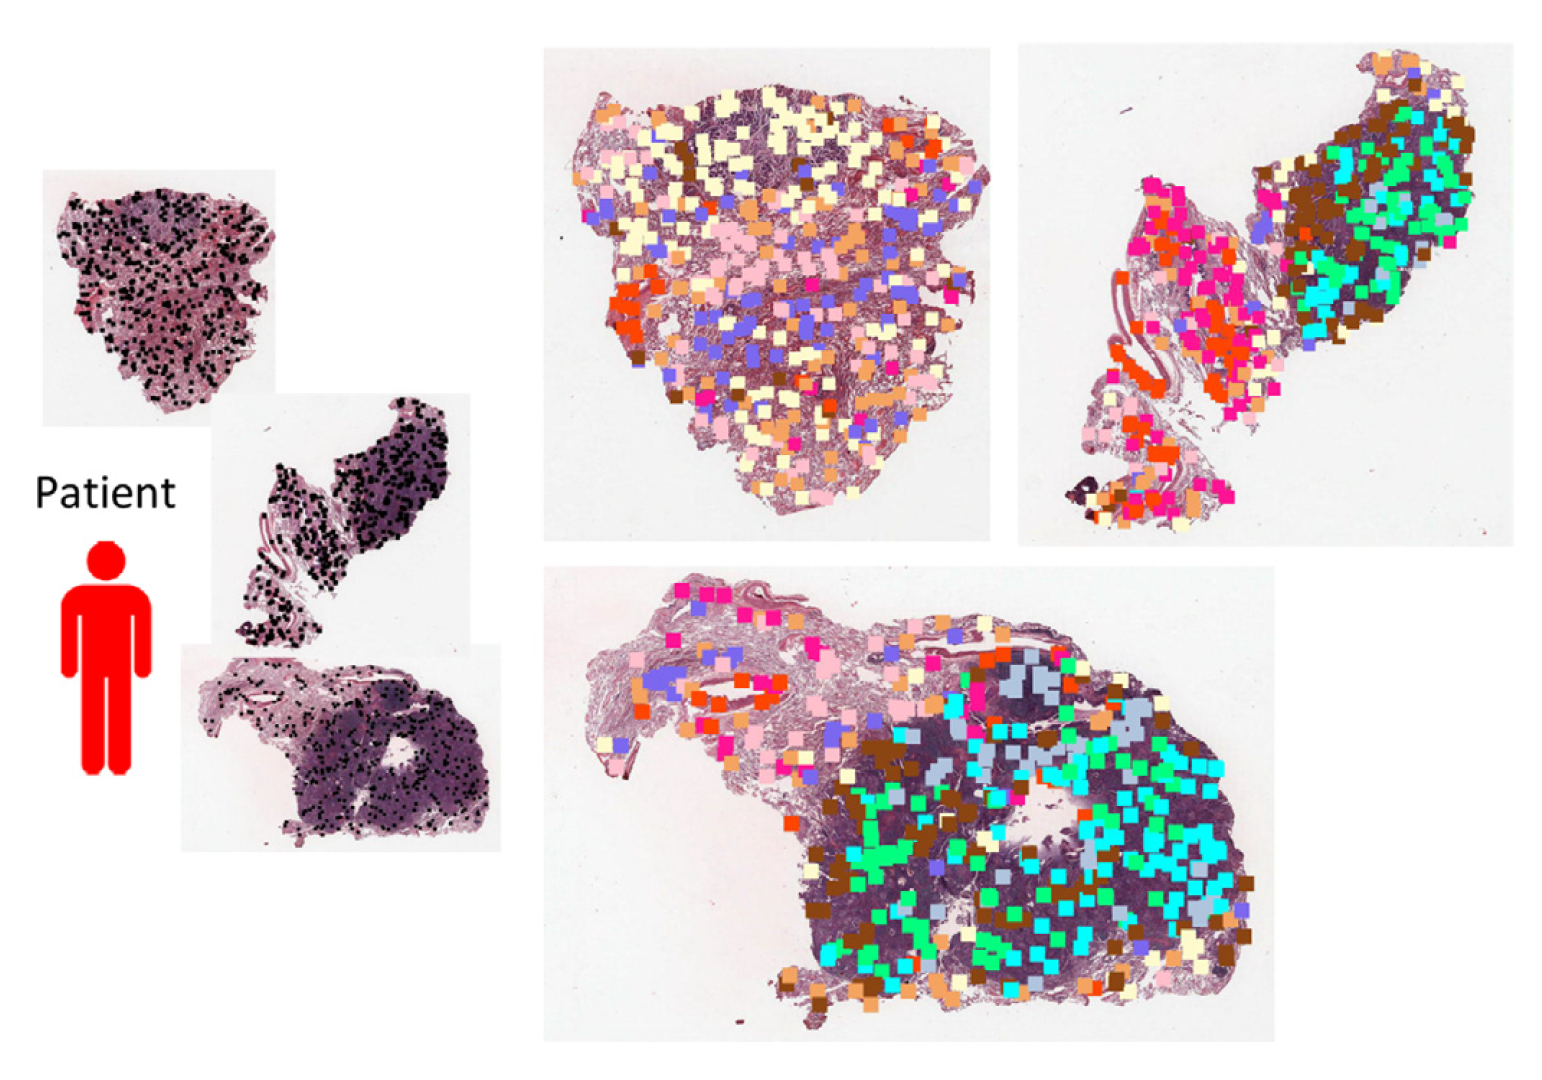
\includegraphics[scale=0.14]{figures/cluster.png}
			\caption{Clustered patches: patches with the same color belong to the same instance.}
			\label{fig:cluster}
		\end{figure}
	\end{frame}

	\begin{frame}
		\frametitle{DeepAttnMISL}
		Contributions (cont.)
		
		\begin{table}[H]
			\begin{center}
				\begin{tabular}{ | l | r | r | r | }
					\hline
					& NLST & MCO\_130K & MCO\_1M \\
					\hline
					Patients & 387 & 1146 & 1146 \\
					\hline
					WSIs & 1177 & 1614 & 1614 \\
					\hline
					Patches & 275244 & 132910 & 915324 \\
					\hline
					Patches/WSI & 234 & 82 & 567 \\
					\hline
				\end{tabular}
			\end{center}
			\caption{The numbers of patients, WSIs, patches and the average number of patches per WSI.}
		\end{table} 
	\end{frame}

	\begin{frame}
		\frametitle{DeepAttnMISL}
		Methodology
		
		\begin{itemize}
			\item Overview \\
			\vspace{5mm}
			Suppose there is a group of patients, $\{ X_i \}, i = 1, \dots, N$ and each of them has a follow-up label $( t_i, \delta_i )$. When $\delta_i = 1$ then $t_i$ is uncensored survival time or failure time, otherwise, $t_i$ is censored survival time.
			
			When dealing with the prognosis problem using multiple instance learning (MIL), a patient is regarded as a bag of instances that $X = \{ x_1, x_2, \dots, x_C \}$, where $C$ denotes the number of instances and may be different for different patients. On the other hand, each instance is a set of patches sampled from WSIs.
		\end{itemize}
	\end{frame}
	
	\begin{frame}
		\frametitle{DeepAttnMISL}
		Methodology (cont.)
		
		\begin{itemize}
			\item Sampling and clustering \\
			\vspace{5mm}
			For each patient, patches are randomly extracted from the WSIs and then clustered into different instances. The 20X pathology images are used for extraction and the patches are of the size $500 \times 500 \times 3$. Then pre-trained deep learning model, such as InceptionV3 and VGG-16, from ImageNet is used for extracting features from the patches. After that, the features are used for clustering the patches using $k$-means clustering. In the proposed multiple instance learning framework, each cluster is considered as an instance.
		\end{itemize}
	\end{frame}

	\begin{frame}
		\frametitle{DeepAttnMISL}
		Methodology (cont.)
		
		\begin{itemize}
			\item Siamese MI-FCN \\
			A siamese multiple instance fully convolutional network (MI-FCN) is developed to extract features from the instances. The weights of each MI-FCN are shared among all the MI-FCNs. For the $i$th patient, $m_i$ features are fed into the MI-FCN to get the instance-level feature $\mathbf{ r }_i$.
			\item Aggregation via attention-based MIL pooling layer
			Let $R = \{ \mathbf{ r }_1, \dots, \mathbf{ r }_C \}$ be the set of instance-level features. Then patient-level feature is aggregated based on the proposed attention mechanism that 
			\[
			\mathbf{ z } = \sum_{ k = 1 }^{ C } a_k \mathbf{ r }_k,
			\] 
			where $a_k = \frac{ \exp \{ \mathbf{ w }^T \tanh( \mathbf{ V }\mathbf{ r }_k^T ) \}}{ \sum_{ j = 1 }^{ C }\exp \{ \mathbf{ w }^T \tanh( \mathbf{ V }\mathbf{ r }_j^T ) }$, and $\mathbf{ w }$ and $\mathbf{V}$ are weights trained in the neural network.
		\end{itemize}
	\end{frame}
	
	\begin{frame}
		\frametitle{DeepAttnMISL}
		Methodology (cont.)
		
		\begin{itemize}
			\item Loss function \\
			\vspace{5mm}
			Partial likelihood function of the Cox proportional hazards model is used as loss function.
		\end{itemize}
	\end{frame}
	
	\begin{frame}
		\frametitle{DeepAttnMISL}
		Experiments
		
		\begin{itemize}
			\item Data description \\
			\vspace{5mm}
			The NLST datasets have both CT and pathology images of lung cancer patients and the MCO study has a collection of clinical and pathological data and pathology images of more than 1500 patients who had colorectal tumor surgery.
			\item Implementation details \\
			\vspace{5mm}
			Adam  optimization is applied with weight decay $5 \times 10^{ -4 }$ and learning rate $10^{ -4 }$. Harrell's c-index and area under the ROC curve (AUC) are used as performance metrics.
			\item Comparisons (MCO dataset) \\
			\vspace{5mm}
			The proposed model is compared with DeepMISL, and WSISA frameworks with Lasso-Cox, En-Cox and MTLSA models.
		\end{itemize}
	\end{frame}
	
	\begin{frame}
		\frametitle{DeepAttnMISL}
		Experiments (cont.)
		
		\begin{table}[H]
			\begin{center}
				\begin{tabular}{ c c r r r r }
					\hline
					Method & Settings & $c = 6$ & $c = 8$ & $c = 10$ & $c = 12$ \\
					\hline
					DeepAttnMISL & 130 K & 0.595 & 0.599 & 0.585 & 0.591 \\ 
					& 1 M & \textbf{0.606} & \textbf{0.600} & \textbf{0.603} & \textbf{0.599} \\
					DeepMISL & 130 K & 0.557 & 0.547 & 0.587 &	0.543 \\
					& 1 M & 0.569 & 0.575 & 0.573 & 0.567 \\
					W-MTLSA & 130 K & 0.558 & 0.567 & 0.524 & 0.547 \\
					W-LassoCox & 130 K & 0.552 & 0.546 & 0.503 & 0.523 \\
					W-EnCox & 130 K & 0.552 & 0.545 & 0.504 & 0.522 \\
					\hline
				\end{tabular}
			\end{center}
			\caption{C-indices of the proposed model and WSISA framework with different settings.}
		\end{table} 
		
	\end{frame}
	
	\begin{frame}
		\frametitle{DeepAttnMISL}
		Experiments (cont.)
		
		\begin{table}[H]
			\begin{center}
				\begin{tabular}{ c c r r r r }
					\hline
					Method & Settings & $c = 6$ & $c = 8$ & $c = 10$ & $c = 12$ \\
					\hline
					DeepAttnMISL & 130 K & 0.623 & \textbf{0.640} & \textbf{0.636} & 0.622 \\ 
					& 1 M & \textbf{0.644} & 0.638 & 0.633 & \textbf{0.637} \\
					DeepMISL & 130 K & 0.564 & 0.552 & 0.590 & 	0.547 \\
					& 1 M & 0.570 & 0.587 & 0.579 & 0.576 \\
					W-MTLSA & 130 K & 0.560 & 0.560 & 0.531 & 	0.555 \\
					W-LassoCox & 130 K & 0.531 & 0.541 & 0.495 & 0.495 \\
					W-EnCox & 130 K & 0.532 & 0.544 & 0.497 & 0.496 \\
					\hline
				\end{tabular}
			\end{center}
			\caption{AUC of the proposed model and WSISA framework with different settings.}
		\end{table} 
		
	\end{frame}
	
	\begin{frame}
		\frametitle{DeepAttnMISL}
		Experiments (cont.)
		
		\begin{figure}[H]
			\centering
			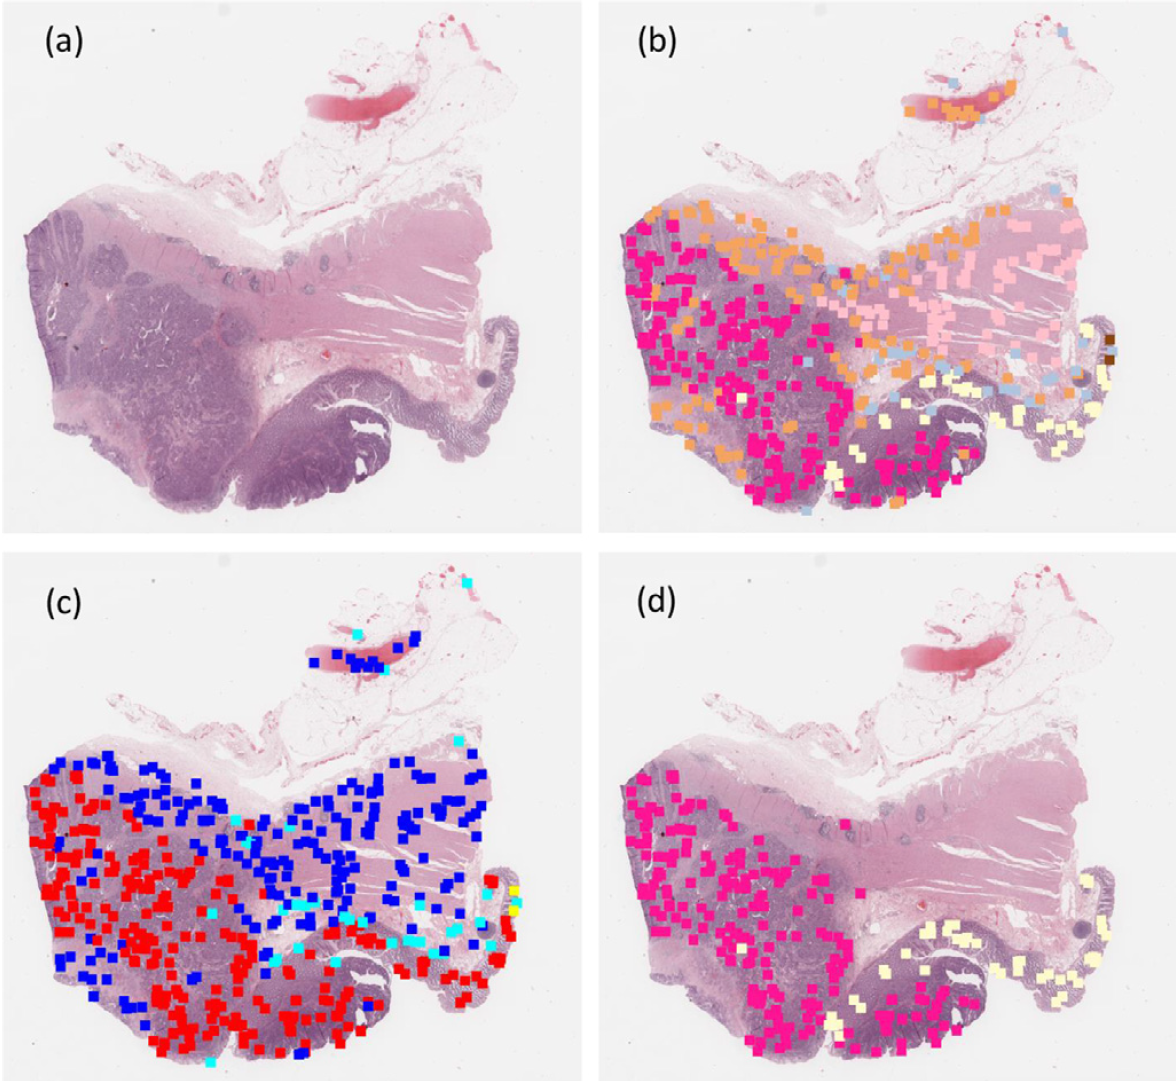
\includegraphics[scale=0.15]{figures/heat1.png}
			\caption{(a) Original WSI, (b) Instance pattern distribution, (c) heatmaps from the proposed model, (d) selected patches with highest attentions.}
			\label{fig:heat1}
		\end{figure}
	\end{frame}
	
	\begin{frame}
		\frametitle{DeepAttnMISL}
		\begin{itemize}					
			\item Comparisons (NLST datasets) \\
		\end{itemize}
		
		\begin{table}[H]
			\footnotesize
			\begin{center}
				\begin{tabular}{ l l r r  }
					\hline
					Type & Method & c-index & AUC \\
					\hline
					Deep Learning & DeepAttnMISL & 0.6963 (0.0660) & 0.7143 (0.0541) \\
					& DeepMISL & 0.6476 (0.0698) & 0.6693 (0.0866) \\
					& Finetuned-WSISA-LassoCox & 0.6123 (0.0216) & 0.6427 (0.0575) \\
					& Finetuned-WSISA-MTLSA & 0.6428 (0.0259) &	0.6963 (0.0668) \\
					& WSISA-LassoCox & 0.5996 (0.0750) &	0.5957 (0.0674) \\
					& WSISA-MTLSA & 0.6305 (0.0575) & 0.6479 (0.0936) \\
					Cox-based & Lasso-Cox & 0.4842 (0.0508)	& 0.4903 (0.1011) \\
					& Cox-boost & 0.5474 (0.0370) & 0.5271 (0.0386) \\
					Parametric & Logistic &	0.4998 (0.0881) &	0.5013 (0.1146) \\
					& Weibull & 0.5577 (0.0395) & 0.5618 (0.0976) \\
					Multi-task based & MTLSA & 0.5053 (0.0509) & 0.5362 (0.0416) \\
					Ranking based & BoostCI & 0.5595 (0.0610) &	0.5487 (0.0532) \\
					\hline
				\end{tabular}
			\end{center}
			\caption{Comparisons of the proposed model and competitors.}
		\end{table} 
	\end{frame}
	
	\begin{frame}
		\frametitle{DeepAttnMISL}
		Experiments (cont.)
		
		\begin{figure}[H]
			\centering
			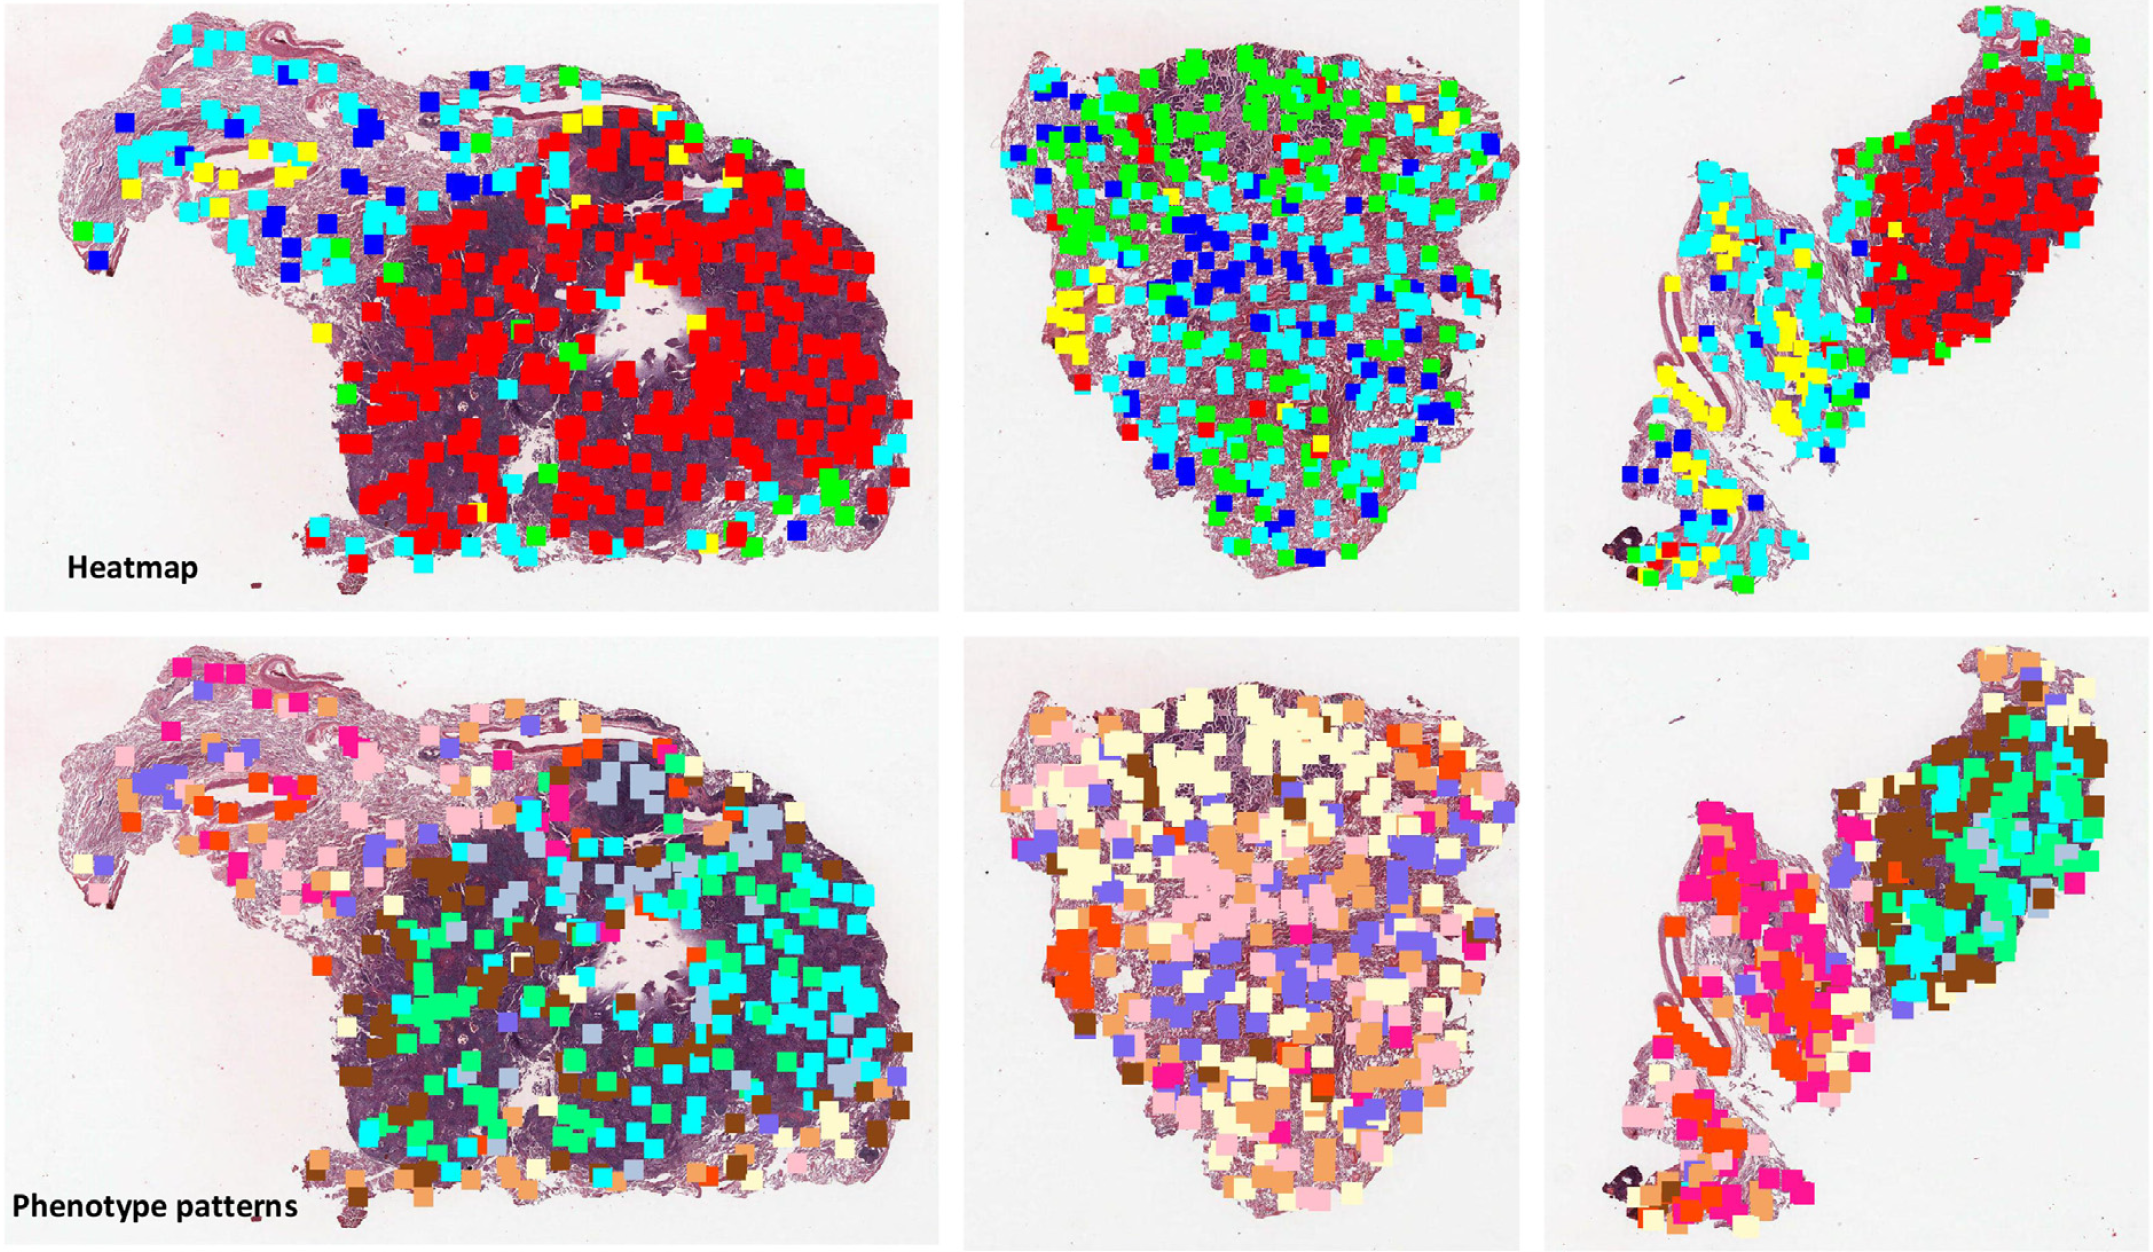
\includegraphics[scale=0.13]{figures/heat2.png}
			\caption{Instance (phenotype) patterns (second row) and the corresponding heatmap (first row).}
			\label{fig:heat2}
		\end{figure}
	\end{frame}
	
	\begin{frame}
		\frametitle{DeepAttnMISL}
		Pros and Cons
		\begin{itemize}
			\item Pros
			\begin{itemize}
				\item The multiple instance learning makes the patches from the same patient share the same patient-level label.
				\item The attention mechanism aggregates the instance-level features to a patient-level feature. The dependency of attention weights on the instance-level features makes the proposed model very flexible that the model is invariant to the permutations of instances.  
			\end{itemize}
			\item Cons
			\begin{itemize}
				\item The details of the sampling procedure of the patches are not discussed. Neither did the variability of the prediction due to the random samples.
				\item The feature extraction and clustering models are not specifically designed for the purpose of prognosis. It is unknown whether the clustering results are meaningful in practice.
			\end{itemize}
		\end{itemize}
	\end{frame}
	
	\begin{frame}
		\frametitle{DeepAttnMISL}
		Pros and Cons (cont.)
		\begin{itemize}
			\item Cons
			\begin{itemize}
				\item Clinical data were not used.
				\item The proposed model still has the limitations of Cox proportional hazards model.
			\end{itemize}
		\end{itemize}
	\end{frame}
	
	\begin{frame}
		\frametitle{SCNN}
		The proposed model, survival convolutional neural networks (SCNNs), extracts features from patches of WSIs and makes highly accurate predictions of survival of cancer patients. The model is also extended to a genomic survival convolutional neural network (GSCNN) which further utilizes the genomic information. The SCNN framework has a patch sampling and a risk aggregation mechanism which alleviates the intratumoral heterogeneity and the inadequate image sample problems. The predicted risk score of the patches can be used for identify prognosis relevant regions in the WSI. Experiments have been conducted on the Cancer Genome Atlas (TCGA) Lower-Grade Glioma (LGG) dataset and Glioblastoma (GBM) dataset.
	\end{frame}
	
	\begin{frame}
		\frametitle{SCNN}
		Methodology
		
		\begin{figure}[H]
			\centering
			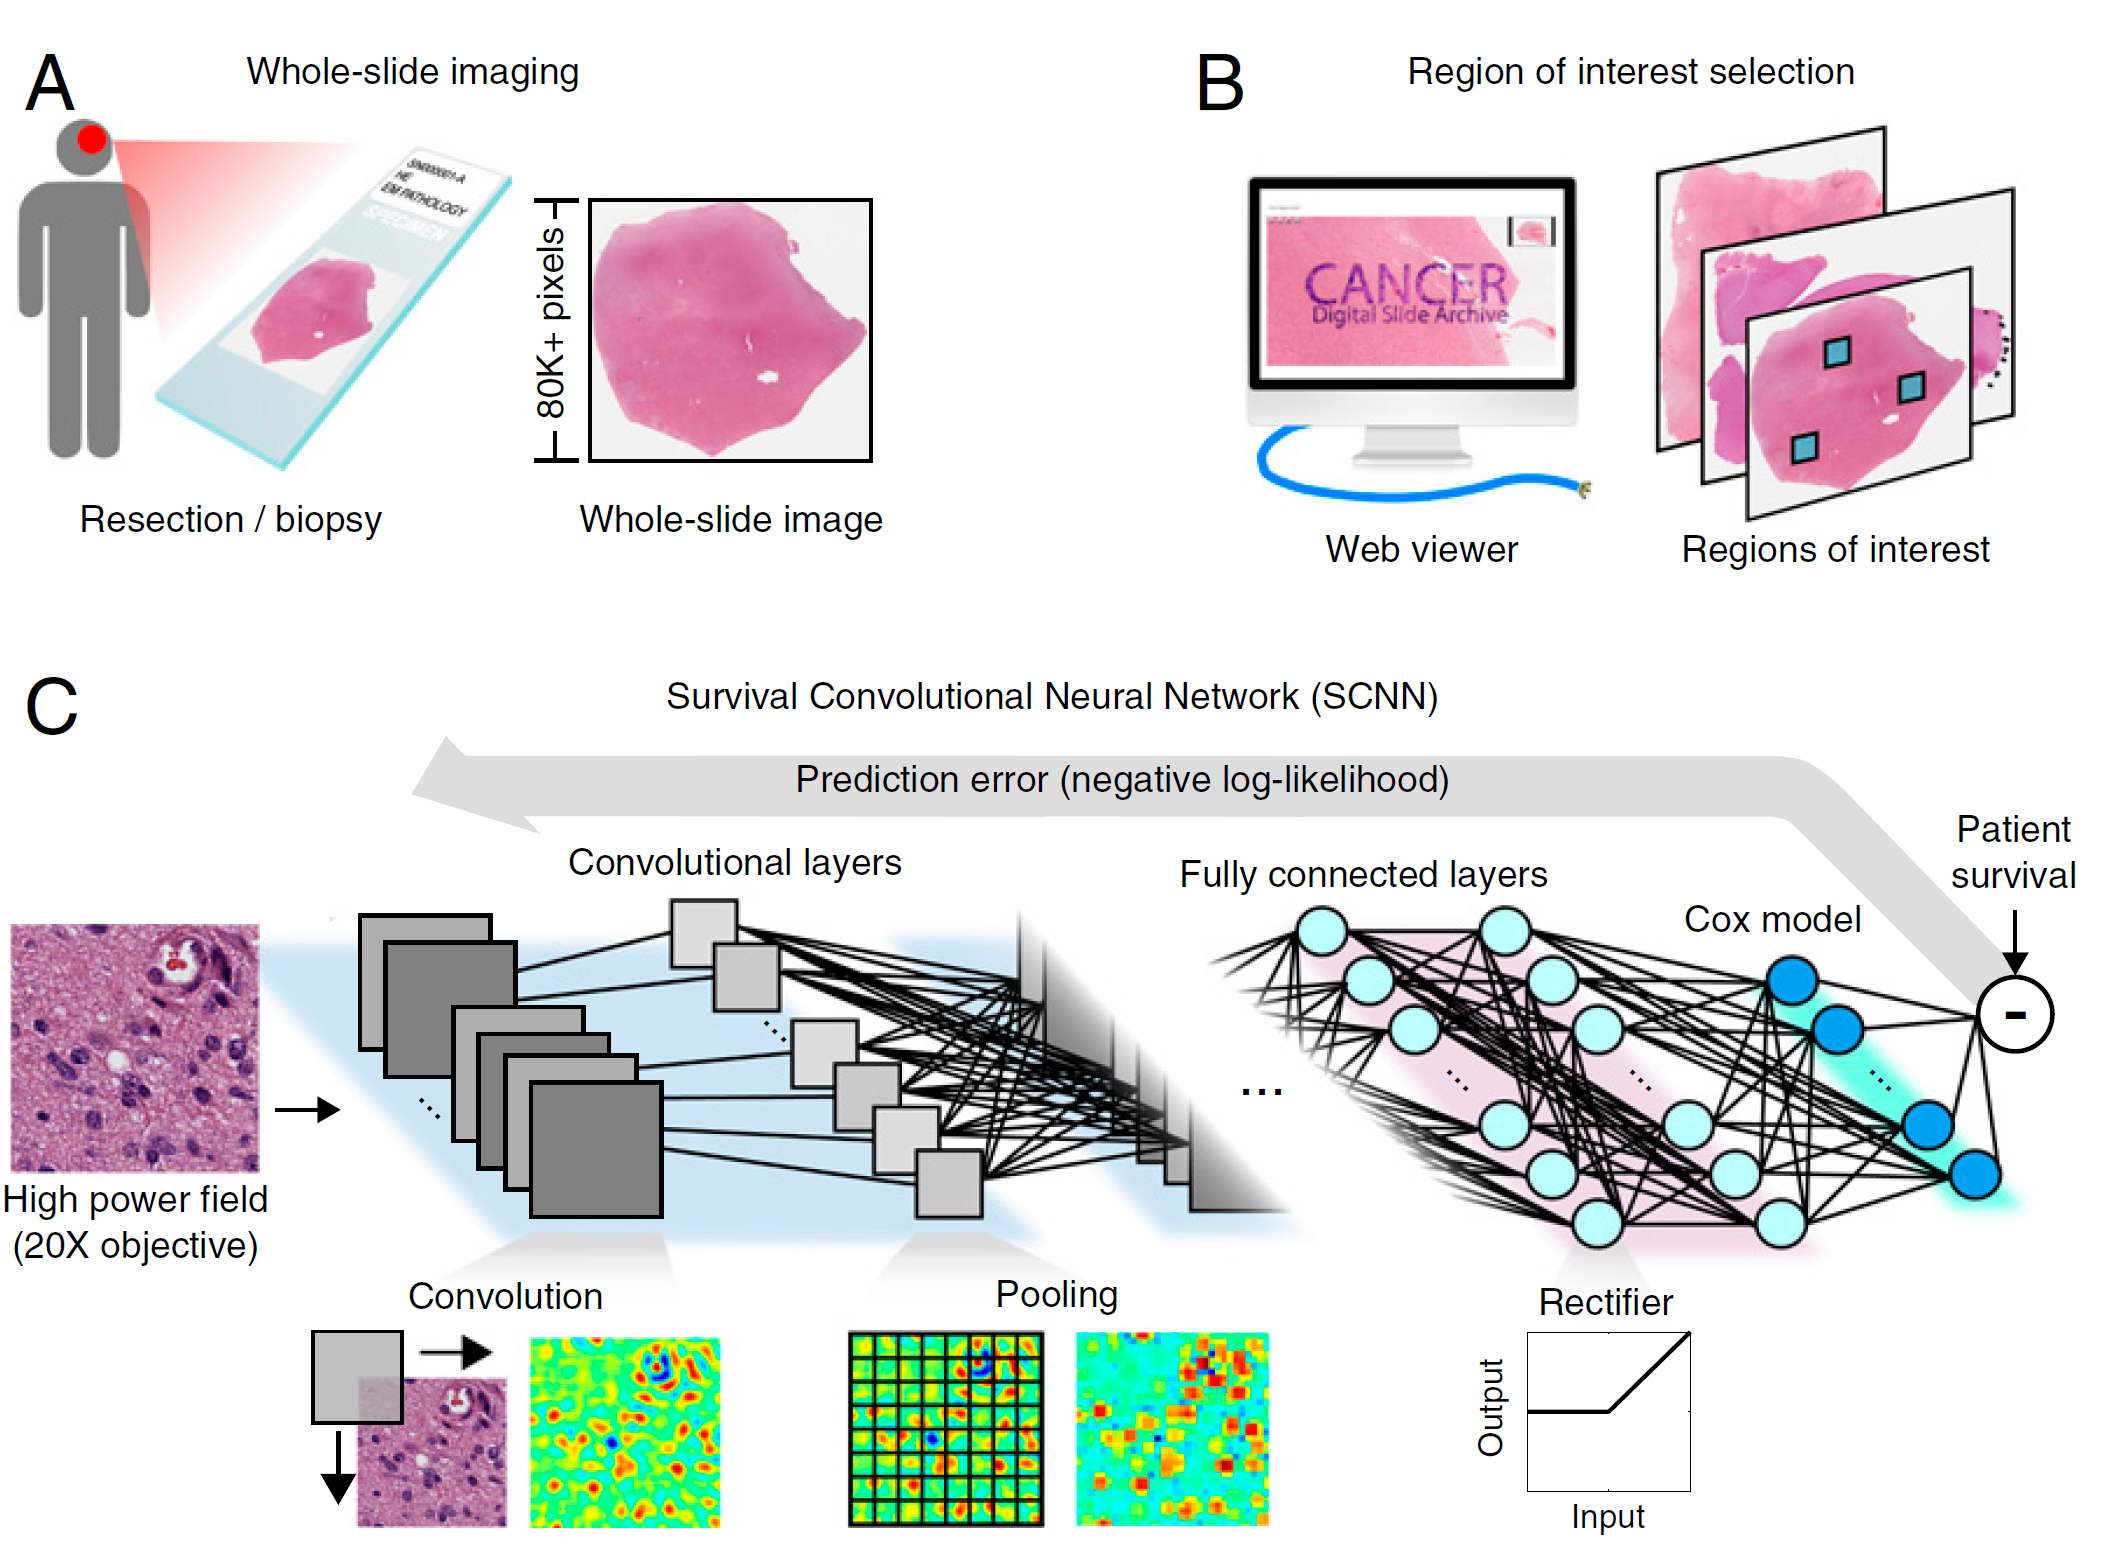
\includegraphics[scale=0.12]{figures/scnn-overall.png}
			\caption{The overall procedure of the proposed framework.}
			\label{fig:scnn-overall}
		\end{figure}
	\end{frame}

	\begin{frame}
		\frametitle{SCNN}
		Methodology (cont.)\\
		\vspace{5mm}
		Overall procedure of the proposed framework
		\begin{enumerate}[A]
			\item Tissue sections of a patient were H\&E stained and scanned to obtain whole slide images.
			\item The representative regions of interest (ROI) were delineated manually by pathologists. 
			\item High power fields (HPFs) were randomly sampled from these ROIs and used to train the SCNN. The SCNN consists of a 19-layer Visual Geometry Group (VGG) convolutional neural network architecture and a Cox proportional hazards model layer. The partial likelihood function was used as loss function.
		\end{enumerate}
	\end{frame}
	
	\begin{frame}
		\frametitle{SCNN}
		Methodology (cont.)
		
		\begin{figure}[H]
			\centering
			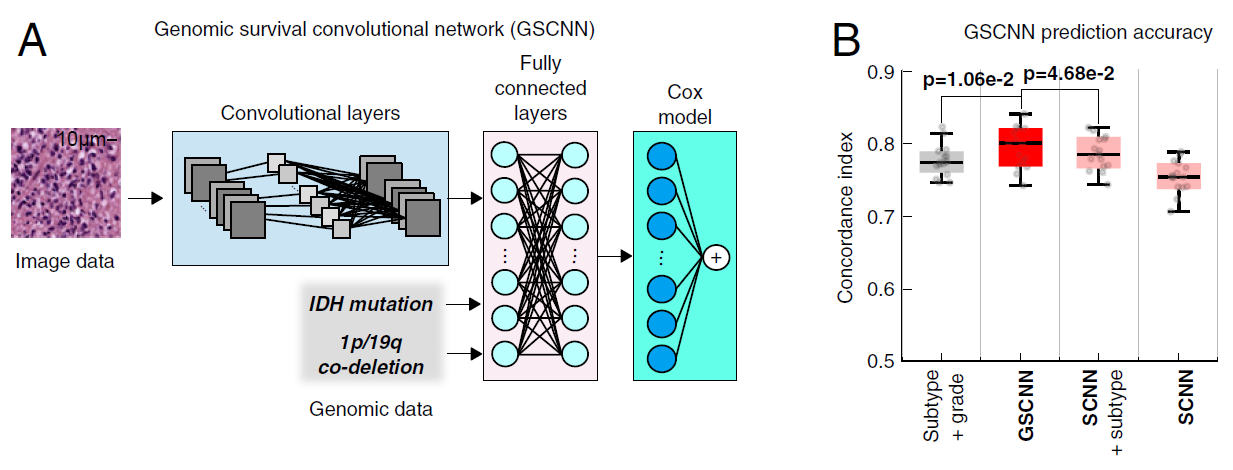
\includegraphics[scale=0.27]{figures/GSCNN.png}
			\caption{Model structure of the GSCNN.}
			\label{fig:gscnn}
		\end{figure}
	\end{frame}

	\begin{frame}
		\frametitle{SCNN}
		Methodology (cont.)
		
		\begin{figure}[H]
			\centering
			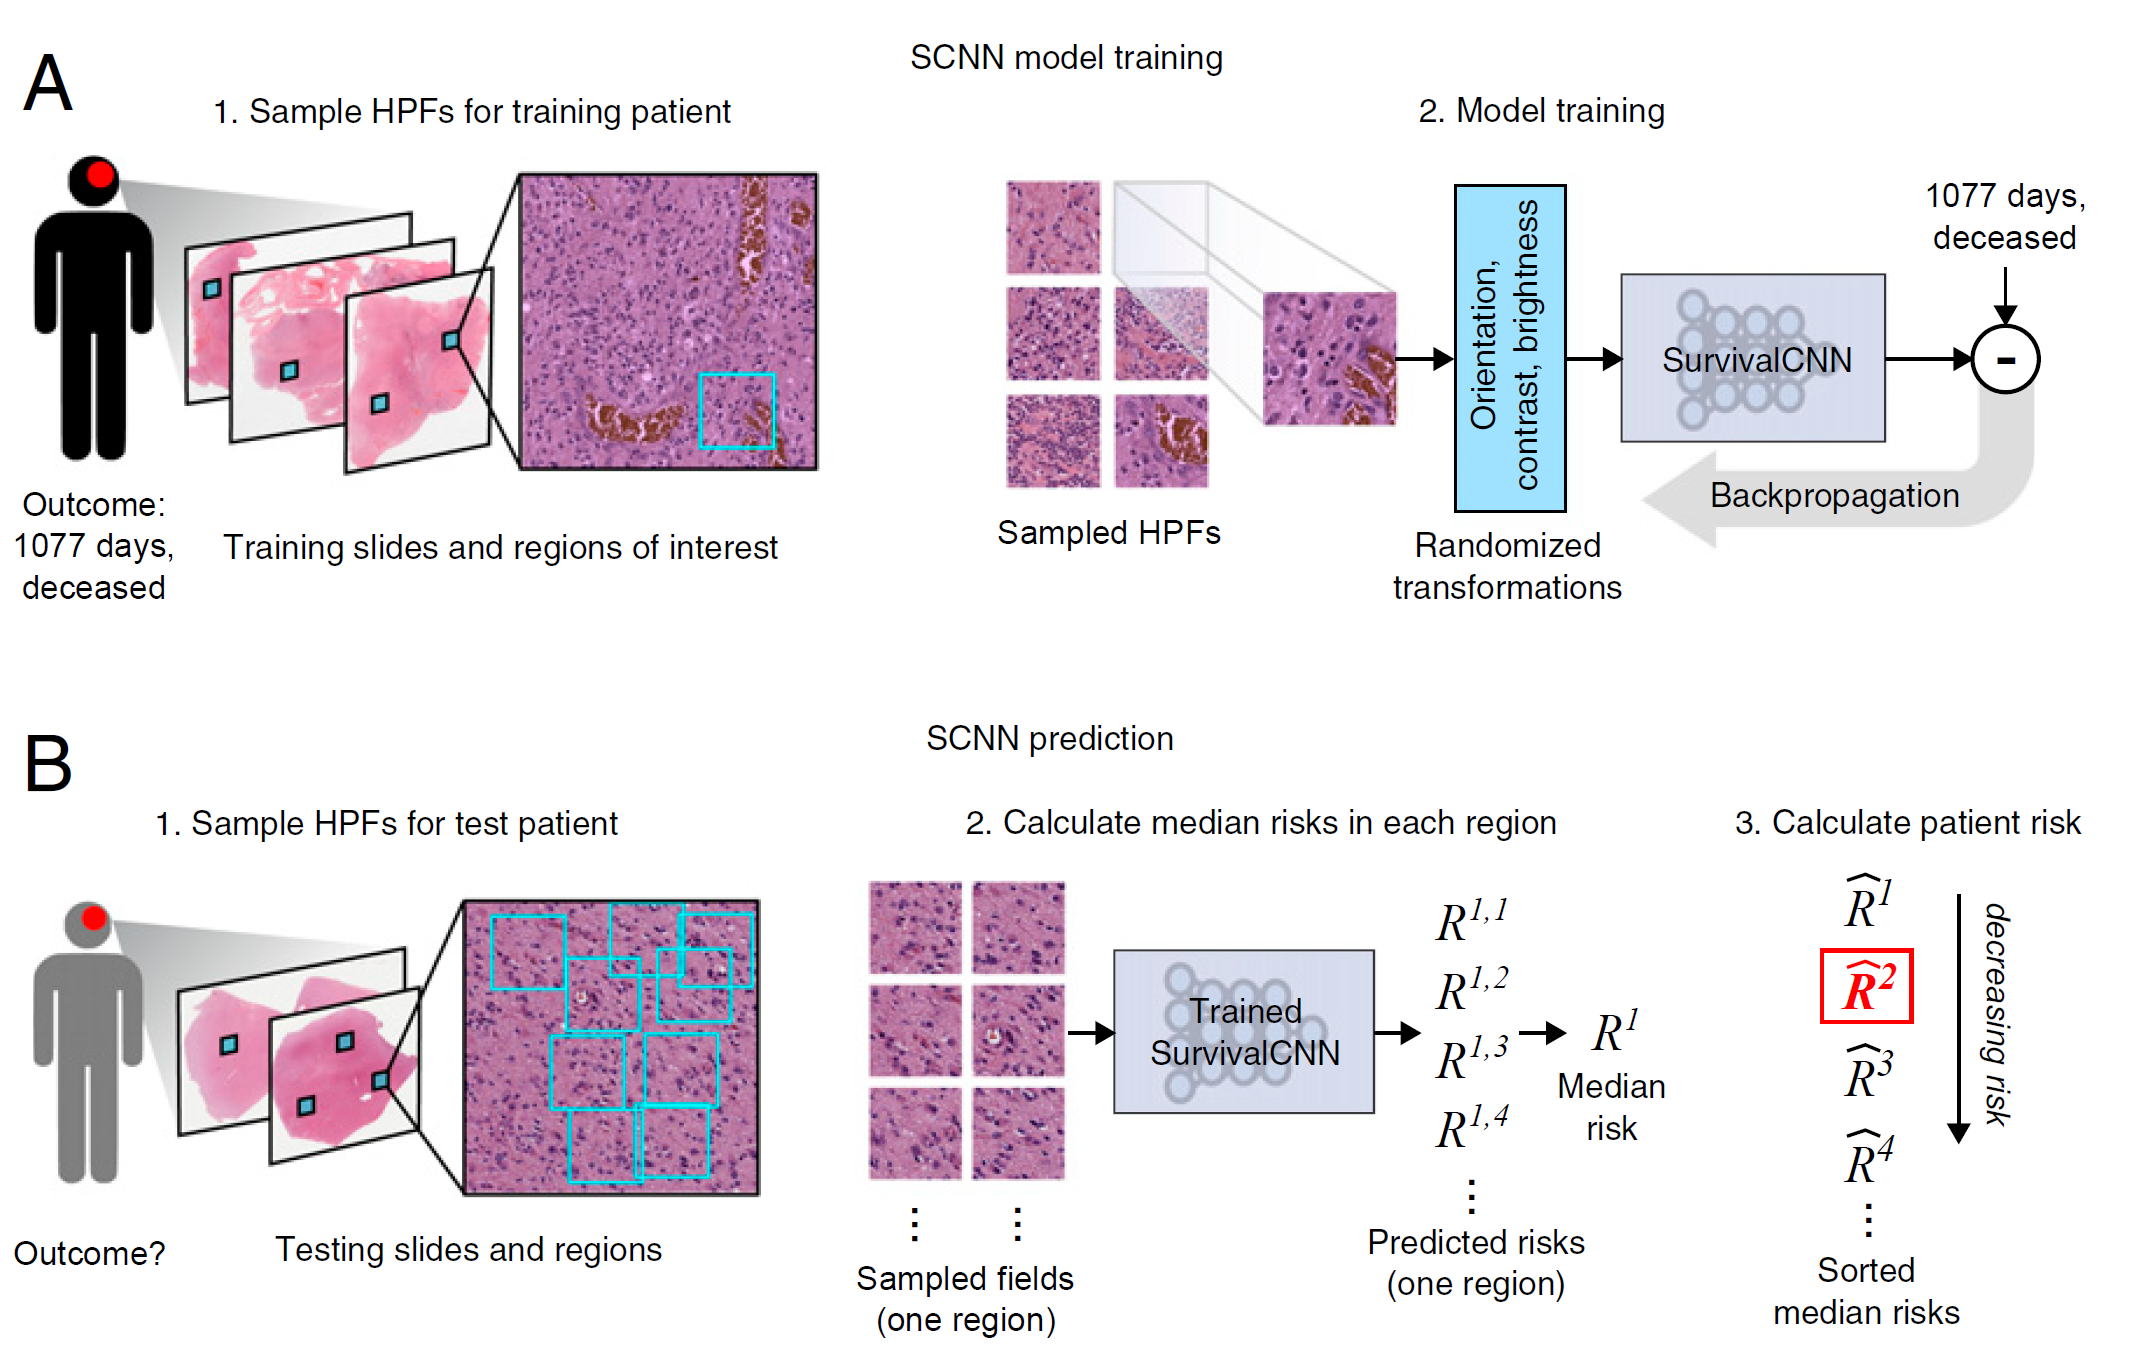
\includegraphics[scale=0.12]{figures/scnn-train-pred.png}
			\caption{The steps in training and predicting.}
			\label{fig:scnn-train-pred}
		\end{figure}
	\end{frame}
	
	\begin{frame}
		\frametitle{SCNN}
		Methodology (cont.)
		\begin{enumerate}[A]
			\item For training the deep neural network, one HPF of the size $256 \times 256$ is randomly sampled from each ROI. As a result, each patient may have multiple HPFs. Then each HPF undergoes random transformations and is fed into the network as an independent observation. In each training epoch, new HPFs are sampled and transformed for training the network.  
			\item When predicting the survival of a new patient, 9 HPFs are sampled from each ROI. Then the risk scores are calculated for those HPFs. The median risk score of the HPFs in a same ROI is used for representing the ROI-level risk score. Next, the ROI-level risk scores are sorted and the second greatest value is regarded as the patient-level risk score. The sampling and filtering steps emulates the manual histologic evaluation procedure that the most malignant region observed within a heterogeneous sample is used for prognostication.
		\end{enumerate}
	\end{frame}
	
	\begin{frame}
		\frametitle{SCNN}
		Experiments
		\begin{itemize}
			\item Data, performance metric and baseline model
			
			The TCGA-LGG and TCGA-GBM datasets were combined instead of being used separately. In total, there were 1061 WSIs of 769 lower-grade glioma and glioblastoma patients. The overall survival was used in the analysis and it ranged from several months to more than 14 years. Besides pathology images, molecular subtype was used in the GSCNN model. Other factors, such as histologic grade, age and sex were also considered when evaluating the proposed models. The Harrell's C index was used as the performance metric. The Cox proportional hazards model with molecular subtype and histologic grades as explanatory variables was used as a baseline model for comparison.
		\end{itemize}
	\end{frame}
	
	\begin{frame}
		\frametitle{SCNN}
		Experiments (cont.)
		
		\begin{figure}[H]
			\centering
			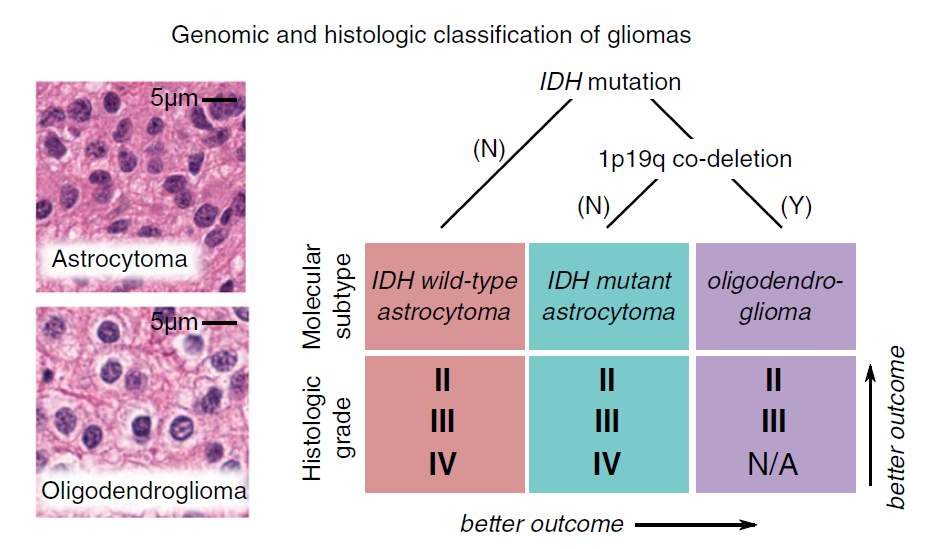
\includegraphics[scale=0.35]{figures/molecular-subtype.png}
			\caption{Examples of molecular subtypes.}
			\label{fig:ms}
		\end{figure}
	\end{frame}
	
	\begin{frame}
		\frametitle{SCNN}
		Experiments (cont.)
		
		\begin{figure}[H]
			\centering
			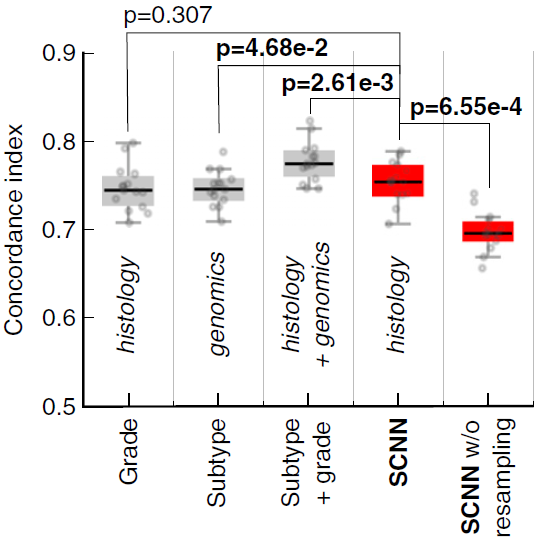
\includegraphics[scale=0.35]{figures/c-index.png}
			\caption{Comparisons among baseline models and SCNNs.}
			\label{fig:c-index}
		\end{figure}
	\end{frame}
	
	\begin{frame}
		\frametitle{SCNN}
		Experiments (cont.)
		
		\begin{figure}[H]
			\centering
			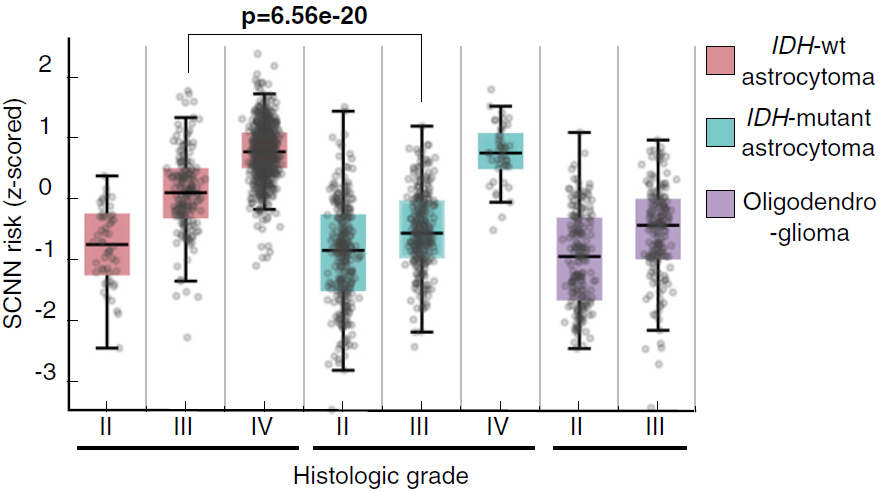
\includegraphics[scale=0.38]{figures/c-index-by-type.png}
			\caption{Risk scores by molecular subtype and histologic grade.}
			\label{fig:ctype}
		\end{figure}
	\end{frame}

	\begin{frame}
		\frametitle{SCNN}
		Experiments (cont.)
		
		\begin{figure}[H]
			\centering
			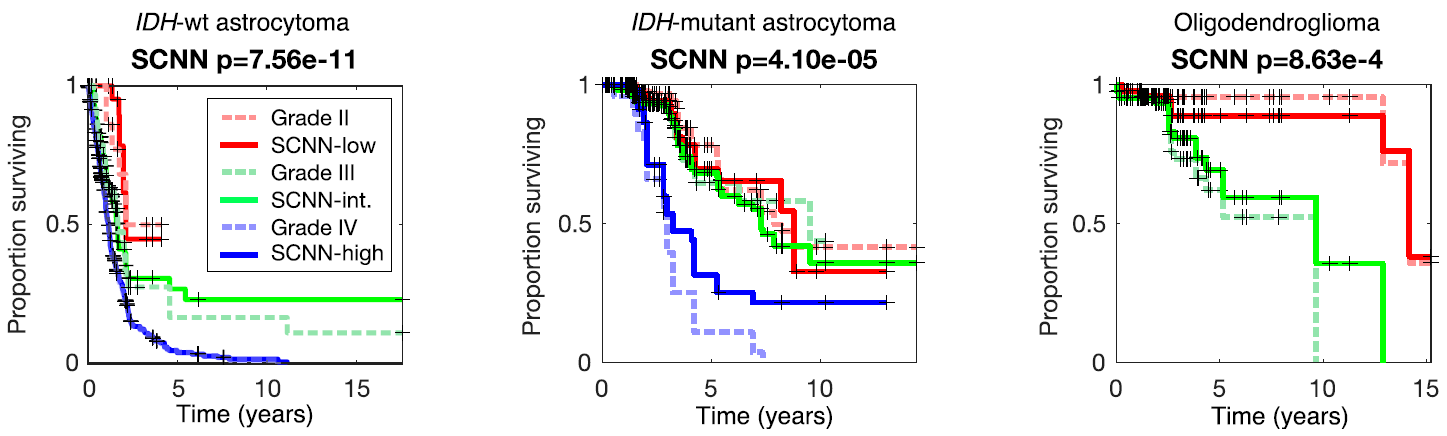
\includegraphics[scale=0.24]{figures/km-curve.png}
			\caption{Grouping based on risk scores from SCNN.}
			\label{fig:km-curve}
		\end{figure}
	\end{frame}

	\begin{frame}
		\frametitle{SCNN}
		Experiments (cont.)
		
		\begin{table}[H]
			\begin{center}
				\begin{tabular}{ l r r r r r }
					& \multicolumn{3}{c}{Single covariate} & SCNN & GSCNN \\
					\cline{2 - 6}
					Variable & c-index & HR & $p$-value & $p$-value & $p$-value \\
					\hline
					SCNN & 0.741 & 7.15 & < 0.05 & < 0.05 & —\\
					GSCNN & 0.781 &	12.60 & < 0.05 & — & < 0.05\\
					IDH-WT & 0.726 & 9.21 & < 0.05 & < 0.05 & 0.93 \\
					IDH-mut & — & 0.23 & < 0.05 & < 0.05 & 0.10 \\
					H-IV & 0.721 & 7.25 & < 0.05 & 0.159 & 0.017 \\
					H-III & — & 0.44 & < 0.05 & 0.082 & 0.024 \\
					Age & 0.744 & 1.77 & < 0.05 & < 0.05 & < 0.05 \\
					Sex(female) & 0.552 & 0.89 & 0.29 & 0.168 & 0.18\\
					\hline
				\end{tabular}
			\end{center}
			\caption{C-indices and $p-$values.}
		\end{table} 
	\end{frame}
	
	\begin{frame}
		\frametitle{SCNN}
		Pros and Cons
		\begin{itemize}
			\item
		\end{itemize}
	\end{frame}

	\begin{frame}[allowframebreaks]
		\begin{singlespace}
			\interlinepenalty=10000	% prevents bib items from splitting across pages
			\bibliography{prognosis-medical}
			\bibliographystyle{apalike}
		\end{singlespace}
	\end{frame}
	
\end{document} 